\chapter{Methods}\label{methods}

For this project, I am interested in two factors that help characterise the cancer mutation profile: genomic location effect (GLE) and sequence context effect (SCE; Figure \ref{fig:workflow}). I examined each factor on two complementary scales: analysis of whole disease (section \ref{methods:gle} and \ref{methods:sce}) and cancer classification for individuals (section \ref{methods:ml}). The former was partly used to interrogate the biological basis for the latter, whereas the latter could validate the patterns detected by the former.

\begin{figure}[h!]
    \centering
    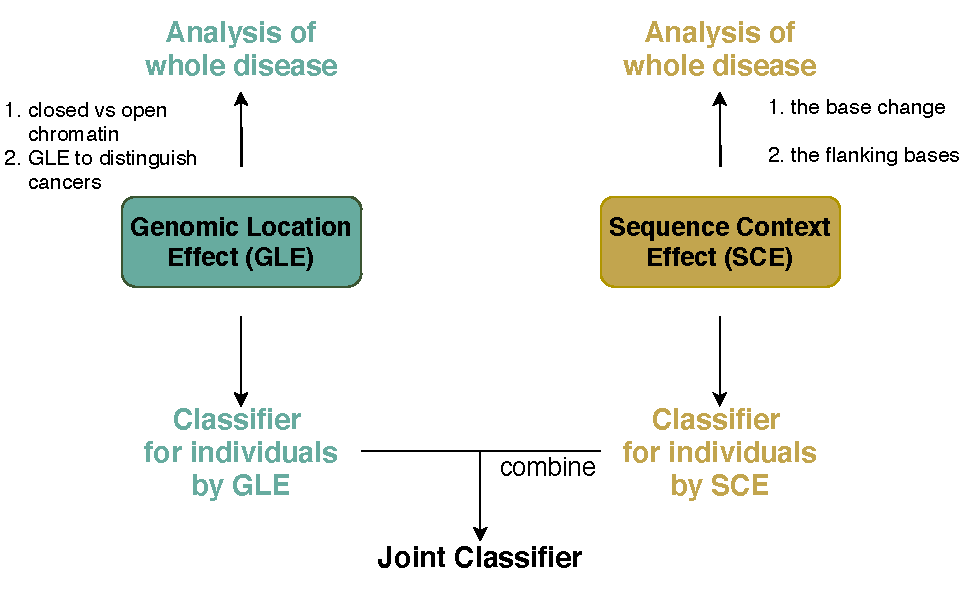
\includegraphics[scale=0.85]{graphics/workflow.pdf}
\caption{}
    % \caption{\textbf{Project workflow for understanding cancer mutagenesis data and exploiting it for cancer classification.} On one hand, cancers were analysed on the whole disease scale, which considered mutations from all donors of the same diseases as a whole. This magnified the signals in the data and made it easier for understanding the mutagenesis process. On the other hand, the information from the factors analysed above was used for training a classifier on the individual donor scale, meaning that this classifier could potentially be applied to a new patient's mutation data to predict their cancer. This followed a standard machine learning training procedure, outlined in Section \ref{methods:ml}.}
    \label{fig:workflow}
\end{figure}


\section{Data description}
\subsection{PCAWG - Mutation data} 
The critical source of data for the project was the mutation data provided by the Pan-Cancer Analysis of Whole Genome (PCAWG) project \citep{Campbell2020}. This data consisted of whole genome sequencing of both cancerous and healthy tissues (mostly blood) for all cancer patients, covering 2658 cancer samples from 28 cancer types. PCAWG relied on contrasting the cancerous against healthy tissues to determine whether a mutation was a \gls{sommut}. Mutations were identified by combining three established pipelines (Sanger \citep{Jones2016CgpCaVEManWrapper:Data}, EMBL/DKFZ \citep{Rimmer2014IntegratingApplications}, and Broad \citep{Cibulskis2013SensitiveSamples}).

This project was limited to analysing somatic \glspl{point_mut}. I sampled 12 cancers whose DHS data for the putative original cells was also available (Table \ref{tab:encode}). A summary of the mutations for the 12 cancers can be found in the appendix (Table \ref{tab:mutation_summary}, Figure \ref{fig:mutation_summary}). Mutation data for all individuals and all mutations was downloaded as a MAF file from the \href{https://dcc.icgc.org/releases/PCAWG/consensus_snv_indel}{International Cancer Genome Consortium (ICGC)}. Driver mutations were filtered out based on \href{https://dcc.icgc.org/releases/PCAWG/driver_mutations}{the PCAWG's driver mutation project} because driver mutations are under selection pressure and have different mutation rates to passenger mutations. Selection pressure was a confounder as the question of interest concerned the informativeness of the mutagenesis process. The information this project utilised from PCAWG was the mutations, their genomic locations, their donor ID and the donor's cancer. 

\subsection{Reference genome} 
To reconstruct the cancer genome, both mutation data and a standard human reference genome are required. The human reference genome was downloaded from the \href{http://hgdownload.soe.ucsc.edu/goldenPath/hg19/chromosomes}{UCSC genome browser}. As PCAWG used Human Genome Assembly 37, the same version of genomic coordinates was used for this project. As an additional check, I also established that the wildtype base at each mutated position and its local reference sequence context provided by PCAWG matched the sequence at that position from the reference genome. 

\subsection{DHS data for chromatin status} 
Part of my project investigated the relationship between mutation distribution and chromatin status. Based on literature search, I identified the most likely tissue of origin for the cancer of interest. These are summarised in Table \ref{tab:encode}. DNase I hypersensitivity (DHS) data for these tissues of origin, as a canonical measure for chromatin status, was from the ENCODE study \citep[downloaded from either \href{https://genome.ucsc.edu/cgi-bin/hgFileUi?db=hg19&g=wgEncodeOpenChromDnase}{Duke} or \href{https://genome.ucsc.edu/cgi-bin/hgFileUi?db=hg19&g=wgEncodeUwDnase}{UW};][]{Thurman2012TheGenome,Klemm2019ChromatinEpigenome}. Specifically, ENCODE measured the level of Dnase hypersensitivity across the genome and identified Dnase hypersensitive regions based on a threshold set by an established algorithm \citep{Boyle2008High-ResolutionGenome}. I used ENCODE identification of Dnase hypersensitive spatial ranges in the genome as open chromatin regions and the rest of the genome as closed chromatin regions.

\section{Algorithm development}
\subsection{Reproducibility} 
\href{http://git-scm.com}{Git} was used as a Version Control tool. Accordingly, the entire code history has been recorded and stored on \href{https://github.com}{GitHub}.

The entire project was done in loops, which means that most analyses were repeated on increasing scales. This not only increased the opportunity for code efficiency to be improved but also helped ensure that the algorithms are reproducible. 

The code projects are available in \\ \url{https://github.com/GavinHuttley/PhuongAnalysis}, \url{https://github.com/GavinHuttley/PhuongData}, \url{https://github.com/GavinHuttley/PhuongLibrary} \\ and \url{https://github.com/GavinHuttley/PhuongR}. \\ All code is available upon request for now, but will be made public when more thorough testing is complete. 

\subsection{Developing packages}
Most core functions were written in Python v3.8.6 \citep{van1995python}, with visualisation and some analyses written in R v4.1.0 \citep{r}. Python libraries directly involved in data analysis were \texttt{numpy} v1.20.0 \citep{harris2020array}, \texttt{scipy} v1.6.0 \citep{2020SciPy-NMeth}, \texttt{sklearn} v0.24.2 \citep{scikit-learn}, \texttt{cogent3} v2021.5.7a \citep{pycogent3} and \texttt{MutationMotif} v0.3 \citep{Zhu2017}. R libraries directly involved in data analysis were base R, \texttt{pheatmap} v1.0.12 \citep{pheatmap} and packages from the \texttt{tidyverse} collection such as \texttt{ggplot2} \citep{tidyverse}. Code was written as packages that can be installed and utilised by anyone.

All core functions were tested under explicit hypothetical scenarios for correctness before being applied. This process is called unit testing. Each of the analyses required multiple core functions. For each analysis, core functions were combined in one commmand line application \texttt{\href{https://click.palletsprojects.com/en/8.0.x/}{click}} that can be run either in a terminal or a Jupyter Notebook. The \href{https://github.com/HuttleyLab/scitrack}{Scitrack} Python package was applied to these commands so all code, and  data inputs and outputs of the commands were tracked and saved as log files.

\subsection{Parallelisation}
When analysing large data sets, some steps could be considerably time-consuming, particularly the initial data filtering step and the simulation steps. Therefore, for several steps, I have written scripts for code parallelisation based on the original command line functions. For example, for an analysis that executes the same processes multiple times on independent data objects, the objects were ``distributed'' across different computer cores instead of being processed sequentially on a single computer. Parallelisation was done using OpenMPI \citep{gabriel04:_open_mpi} and \texttt{mpi4py} \citep{Dalcin2011ParallelPython}. This was performed using resources provided by the National Computational Infrastructure Australia.


\section{Whole disease analysis of GLE}\label{methods:gle}

The variation in chromatin structures of different cell types is believed to shape where mutations occur in the genome, giving rise to the genomic location effects (\gls{gle}) that are characteristic of cancers \citep{Polak2015}. The methods in this section serve two purposes: to formally test the presumed biological connection between chromatin structure and mutation locations, and to weigh the importance of GLE as a characteristic of the cancer mutation profile irrespective of the its driving mechanism.  

\subsection{Visualising DHS by multi-dimensional scaling}\label{methods:encode_pca}
Before establishing the relationship between mutation location and chromatin structure, I examined whether and how the relevant original cells were related in terms of chromatin structure using DHS data. The rationale was that if chromatin structure was a true determinant of mutation location, then tissues that were epigenetically similar should have roughly similar patterns of GLE. Furthermore, such similarity might interfere with the informativeness of the GLE as a predictor of cancer when training the classifier.

For each pair of cell types, the intersections of their open chromatin regions were identified. The difference between the pair was then calculated as:

\begin{equation}
    d = 1 - \frac{2i}{o_1 + o_2}
\end{equation}

where $d$ is the difference/distance, $i$ is the total lengths of the genomic regions covered by the intersections, $o_1$ and $o_2$ are the length of the open chromatin regions. Essentially $d$ is the ``complement'' of the ratio between the intersection $i$ and the average length of the open regions $o_1$ and $o_2$. 

Once the distances for all possible pairs of cell types were obtained, I decomposed these distances into their relative coordinates by multi-dimensional scaling. This was done by the R function \texttt{cmdscale}. The coordinates for the 3 most informative dimensions are reported in Figure \ref{fig:encode_pca}, Subsection \ref{gle:pca} of Chapter \ref{gle}.

\subsection{Mutation location in relation to chromatin status}\label{methods:chromatin}
To establish the relationship between the mutation location of a cancer and the chromatin status of its original cell type, I sorted mutations into open and closed chromatin regions as per Figure \ref{fig:gle_workflow}. I then used (1) the G-test for whether we could reject the null that mutations occur without any preference for closed or open regions and (2) the odds ratio statistic to measure the bias towards closed regions.

\begin{figure}[h!]
    \centering
    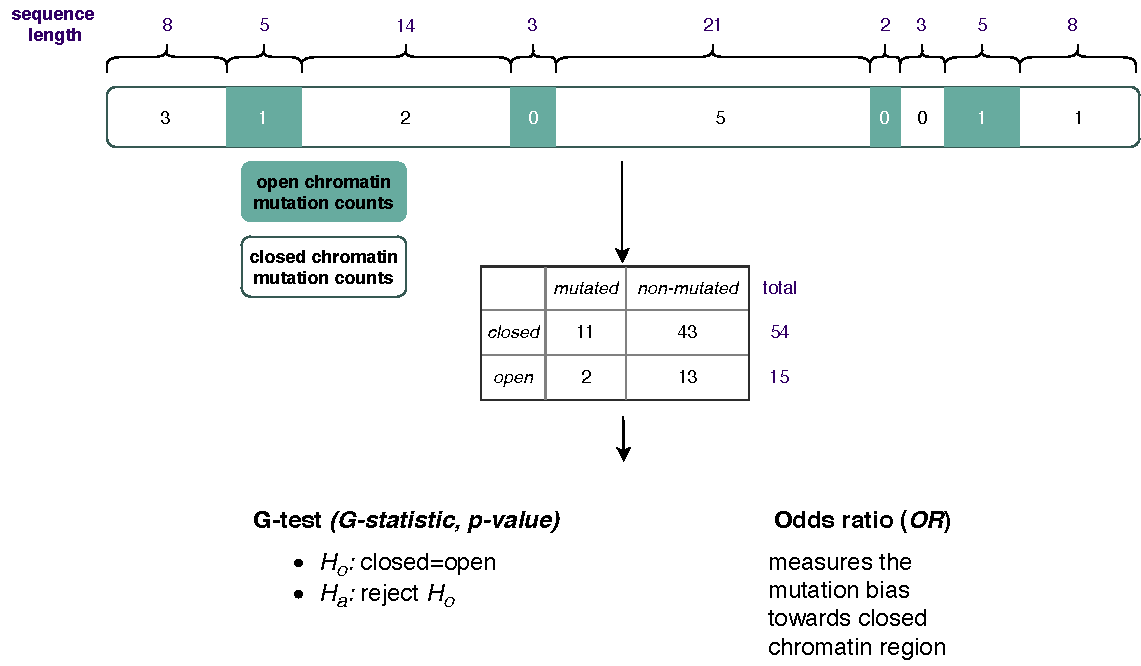
\includegraphics[scale=0.82]{graphics/mutdistribution.pdf}
\caption{}
    % \caption{\textbf{Establishing the relationship between cancer mutation and chromatin structure of the original cell type.} Mutations were sorted into open and closed regions to make a contingency table, from which a G-test can be performed and an Odds-ratio ($OR$) statistic can be calculated. The G-test establishes whether there is a significant bias in mutation location; $OR$ measures the degree of bias towards closed chromatin regions.}
    \label{fig:gle_workflow}
\end{figure}


\subsubsection{Homogeneity test for mutation location between closed and open regions}
I used the G-test of independence \citep{McDonald2014GtestStatistics} to examine the hypothesis whether the distribution of mutations are random across the genome. More formally:

\begin{itemize}
    \item $H_o (Null)$: Mutation abundance is independent of the chromatin status
    \item $H_a (Alternate)$: Mutation abundance is biased by the chromatin status
\end{itemize}

First, the expected number of observations for each cell assuming the null was true was calculated as per Table \ref{tab:count_exp_demo}. For example, the expected number of mutated bases in the closed regions $e_i$ is proportional to the number of bases available in the closed regions $c$ and the number of mutations $m$. The departure of the observed count $o_i$ from the expected $e_i$ was measured by the $G$ statistic, calculated as:
\begin{equation}
    G = 2 \underset{i}{\sum} o_{i} \ln \frac{o_{i}}{e_{i}}
    \label{eq:g}
\end{equation}
where $o_{i}$ are the observed values (\textit{i.e.} entries from Table \ref{tab:count_obs_demo}) and $e_{i}$ are the expected values (\textit{i.e.} entries from Table \ref{tab:count_obs_demo}) and the p-values were obtained by contrasting $G$ against the $\chi^2_1$ distribution. I used Bonferroni method on the p-values for multiple test correction as per equation \ref{eq:bonferroni} in the Appendix \citep{Armstrong2014WhenCorrection}.

\vspace{0.2cm}
\begin{table}[ht!]
\caption{}
    % \caption{Demo contingency tables. Panel (a) contains the observed counts, each of the entries $c_m$, $c_n$, $o_m$ and $o_n$ represents an $o_i$ in equation \ref{eq:g}. Panel (b) contains the expected counts, each of the elements represents an $e_i$ in equation \ref{eq:g}.}
    \begin{subtable}[!h]{.5\textwidth}
        \centering
        \begin{tabular}{r|rr|r}
             & Mutated & Non-mutated & Total  \\
        \hline
            Closed & $c_m$ & $c_n$ & $c$ \\
            Open & $o_m$ & $o_n$ & $o$ \\
        \hline    
             & $m$ & $n$ & $t$ \\
        \end{tabular}
        \vspace{0.2cm}
    \subcaption{Observed counts}
    \label{tab:count_obs_demo}
    \end{subtable} 
    \quad % for side by side tables
    \begin{subtable}[!h]{.5\textwidth}
        \centering
        \begin{tabular}{r|rr|r}
             & Mutated & Non-mutated & Total  \\
        \hline     
            Closed & $c*m/t$ & $c*n/t$ & $c$ \\
            Open & $o*m/t$ & $o*n/t$ & $o$ \\
        \hline    
             & $m$ & $n$ & $t$ \\
        \end{tabular}
        \vspace{0.2cm}
    \subcaption{Expected counts}
    \label{tab:count_exp_demo}
    \end{subtable}    
\end{table}

\subsubsection{Odds ratio for the bias in GLE}
To complement the G-test, I used the odds ratio \citep[$OR$;][]{Hoppe2017OddsRatios} as a measure of preference for mutations to occur in closed chromatin regions compared to open regions. The formula for $OR$ of the contingency Table \ref{tab:count_obs_demo} is as follows:

\begin{equation}
    OR = \frac{c_m/c_n}{o_m/o_n}
    \label{eq:or}
\end{equation}

where $c_m$, $c_n$, $o_m$ and $o_n$ are all observed values that comes from Table \ref{tab:count_obs_demo}.

\subsubsection{Jackknife for the variation of $OR$}
It is worth noting that even within one cancer type, different donors might vary in the number of mutations they carry and the locations of the mutations (\textit{e.g.} if they are an outlier). If a donor has a very distinctive mutation pattern, their data might bias the $OR$ statistic for their whole cancer cohort, especially when the cohort is small. To address this, I performed a jackknife analysis on this measure for each disease \citep{Miller1974TheReview}. An illustration of the jackknife workflow is shown in figure \ref{fig:jackknife_demo}. Specifically, to see how influential a donor $i$ is on $OR$, I removed that donor, recomputed $OR_i$ and computed a pseudo-value for $OR$ as per equation \ref{eq:jackknife}. 

\begin{equation}
    OR^{pseudo}_i = nOR - (n-1)OR_i
    \label{eq:jackknife}
\end{equation}
where $OR^{pseudo}_i$ is the jackknifed pseudo-value for donor $i$, $OR_i$ is the recomputed $OR$ without donor $i$, $n$ is the number of donors.

Applying this to every donor generates a new set of $OR$ that reflects the potential range of the true $OR$. The result for this is shown in Subsection \ref{gle:or}.

\begin{figure}[h!]
    \centering
    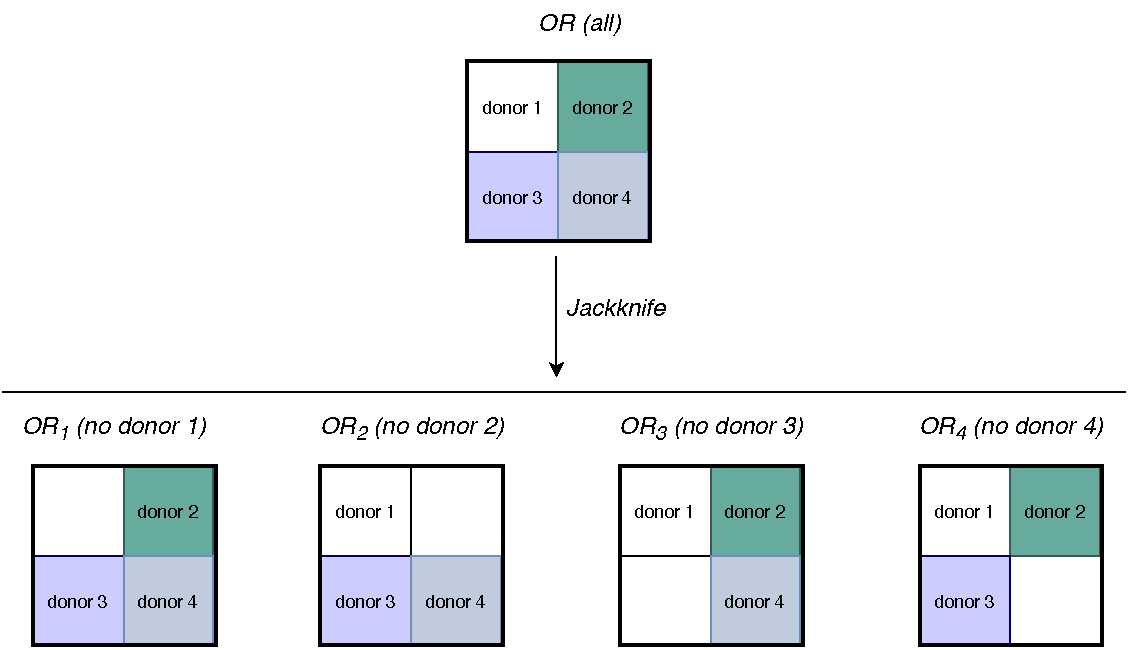
\includegraphics[scale=0.8]{graphics/jackknife_demo.pdf}
\caption{}
    % \caption{\textbf{Illustration of jackknife analysis}. For a hypothetical cancer with 4 donors, the original odds ratio $OR$ was computed. Donor 1 was then omitted and a new odds ratio $OR_1$ was recomputed and a pseudo value $OR^{pseudo}_1$ was obtained. The same was applied to every other donor. The end result was a set of odds ratio statistics $\{OR_1^{pseudo}, \ldots, OR_4^{pseudo}\}$ that were used to estimate the possible range of the true $OR$ statistic}
    \label{fig:jackknife_demo}
\end{figure}


\subsubsection{Mislabelling DHS data}
It is a very natural concern that the calculation of $OR$ is itself biased towards closed chromatin regions purely due to its large size compared to open regions. Besides, if chromatin status is a determinant of mutation location, then cells that have similar DHS should have somewhat similar GLE patterns. To address both of these, I considered all possible combinations of DHS data for the original cell types and mutation data for cancers. Next, instead of calculating $OR$ for the matching DHS/mutation data, I calculated all mislabelled $OR$'s. Eventually, for each cancer, 11 mislabelled $OR$'s and one correctly matched $OR$ were obtained. The result for this is presented in Subsection \ref{gle:mixed_or}.

\subsection{Hypothesis testing of GLE between cancer pairs by bootstrap}\label{methods:bootstrap}

I examined whether GLE could discriminate cancers and what approaches to represent GLE could yield the most resolution. This includes the conventional bin \textit{v.s.} smooth representation and the Wasserstein \textit{v.s.} Euclidean distance measures. 

\subsubsection{Bin \textit{v.s.} smooth representation}
\paragraph{Bin} As briefly described in Figure \ref{fig:mutdistribution_demo}, the bin representation segmented the genome into non-overlapping bins of 1 million bases in length. The number of mutations in each bin was recorded for each chromosome, then divided by the total mutations in that chromosome to get the bin density. 
\paragraph{Smooth} To address the issue with arbitrary boundaries introduced by the discrete bins approach, I proposed a smoothing representation that computes a sliding window of mutation density across each chromosome (Figure \ref{fig:mutdistribution_demo}). This was done using a kernel function \citep[equation \ref{eq:density};][]{Silverman1986DensityAnalysis}. The idea is that the density at a certain location $x$ should be proportional to the distance from $x$ to all other locations $X_i$ where mutations are observed. 

\begin{equation}
    \hat{f}(x) = \frac{1}{nh} \underset{i=1}{\overset{n}{\sum}} K\Big(\frac{x- X_i}{h}\Big)
    \label{eq:density}
\end{equation}

where $\hat{f}$ is the density for location $x$, $n$ is the total number of mutations, $X_i$'s are all genomic locations where mutations occur, $K$ is the kernel function - here the Gaussian kernel was used (appendix equation \ref{eq:gaussian}), $h>0$ is the bandwidth and determines the level of smoothing to be done. Scott's rule \citep[appendix equation \ref{eq:bandwidth};][]{Scott1992MultivariateEstimation} was used to determine the bandwidth. This was done using the python class \texttt{gaussian\_kde} from \texttt{scipy.stats} \citep{2020SciPy-NMeth}.

\subsubsection{Euclidean \textit{v.s.} Wasserstein distance measure}
I separately used the Euclidean \citep{ONeill2006FrameFields} and Wasserstein \citep{Kolouri2017OptimalApplications} distances for both the bin and the smooth representations to compare the GLE from two cancers. The basic difference between two is depicted in Figure \ref{fig:wasserstein_demo}. In a simple sense, Euclidean measures the distance between two densities in a point-wise manner and in the vertical direction while Wasserstein uses both the vertical and horizontal directions. 

\begin{figure}[h!]
    \centering
    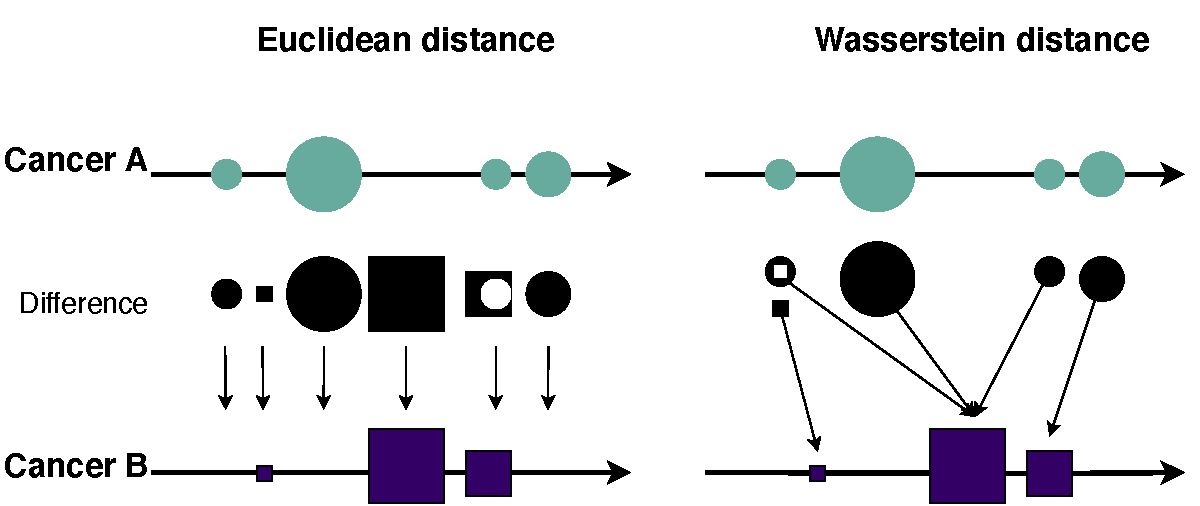
\includegraphics[scale=0.8]{graphics/wasserstein_demo.pdf}
    \caption{\textbf{Schematic diagram for Euclidean and Wasserstein distance between two vectors.} The green circles are data points on the GLE vector for Cancer A, the purple squares are data points on the GLE vector for Cancer B. The black shapes and the arrows combined represent the difference between Cancers A and B. Euclidean is the point-wise difference between the same location on vectors A and B, and is strictly in the vertical direction. In other words, the Euclidean distance between A and B only depends on how different points of similar coordinates are. Wasserstein takes into account both the vertical and horizontal directions; it is intuitively the minimal amount of work required to transport mass from A to B. The Wasserstein distance between A and B depends on both the difference between the magnitude of data points and the path it takes to move data points from A to B.}
    \label{fig:wasserstein_demo}
\end{figure}


\paragraph{Euclidean} The Euclidean distance is also known as the Pythagorean distance. The squared Euclidean distance is the sum of squares of the differences between the two corresponding coordinates of each vector \citep[equation \ref{eq:euclid};][]{ONeill2006FrameFields}.

\begin{equation}
    d_E(a,b) = \sqrt{\sum_{i=1}^n (a_i - b_i)^2}
    \label{eq:euclid}
\end{equation}

where $d_E(a,b)$ is the distance between two vectors $a$ and $b$ that represent the densities of Cancers A and B; $a_i$ and $b_i$ are the $i^{th}$ elements of $a$ and $b$, respectively. This was executed by the python function \texttt{scipy.spatial.distance.euclidean}.

\paragraph{Wasserstein} It is reasonable to view mutation densities as masses of data spatially distributed across a 1-D axis (Figure \ref{fig:wasserstein_demo}). From this viewpoint, Wasserstein appears a well suited measure of distance between two densities. Intuitively, it measures the minimal amount of work required to move mass from Cancer A to B. Mathematically, it does so by searching for the minimum distance with respect to all the joint distributions $\gamma(x,y)$ of random variables $(X,Y)$ that have \glspl{marginal} $a$ and $b$, as follows.

\begin{equation}
    d_W(a,b) = \underset{\gamma \in \mathcal{J}(a,b)}{\inf} \int |x-y|^p d \gamma(x,y) 
    \label{eq:wassertein}
\end{equation}

where $d_W$ is the Wasserstein distance; $a$ and $b$ are the vectors that represent the densities of Cancers A and B, respectively; $\mathcal{J}$ is the set of all joint distributions $\gamma$. (There are infinite joint distributions $\gamma$). The $\gamma(x,y)$ terms represent the transport plans to move data from A to B and the $|x-y|$ term represents the distance to move from A to B based on that transport plan, $p$ is the order of the Wasserstein distance, I used $p=1$. The smallest value that takes into account the two terms (selected by the infimum operator $\inf$) is the Wasserstein distance. The Wasserstein distance assumes that A and B have the same masses, which was satisfied because by definition, the area under the curve for densities is always 1. This was done using the python function \texttt{scipy.stats.wasserstein\_distance}.


\subsubsection{The bootstrap}

Having established the representations and distance measures, the next questions are whether the distance is significantly large enough to conclude that the cancer types have different patterns of GLE, and which representation can extract the most information for doing so. For this, I used the bootstrap method \citep{Singh2010BootstrapMethod}, which is based on random re-sampling. For a pair of cancers A and B, the formal hypotheses are

\begin{itemize}
    \item $H_o (Null)$ GLE for A is the same as B
    \item $H_a (Alternate)$ GLE for A is different from B
\end{itemize}

The bootstrap procedure is illustrated in Figure \ref{fig:bootstrap_demo}. For a pair of cancer types A and B with distance $d$, I first aggregated all mutations from the two cancers to create a pool of mutations. I then simulated 2 imaginary cancers 1 and 2 by randomly drawing mutations from that previously constructed mutation pool. The constraint on the simulation was that the total number of mutations in Cancer 1 had to be the same as either A or B - likewise for Cancer 2. This constraint was so that the simulated cancers are as close to the original as possible. I then measured the simulated distance $d_i$ between 1 and 2. This process was repeated 1000 times. To conclude that A and B are significantly different from each other, $d_{obs}$ should be larger than most of the simulated $d_i$. In the end, the number of the simulated distances that are greater than the observed distance between A and B divided by 1000 was the estimated p-value the hypothesis test. The result for bootstrap hypothesis testing is presented in Section \ref{gle:bootstrap} of Chapter \ref{gle}.

\begin{figure}[h!]
    \centering
    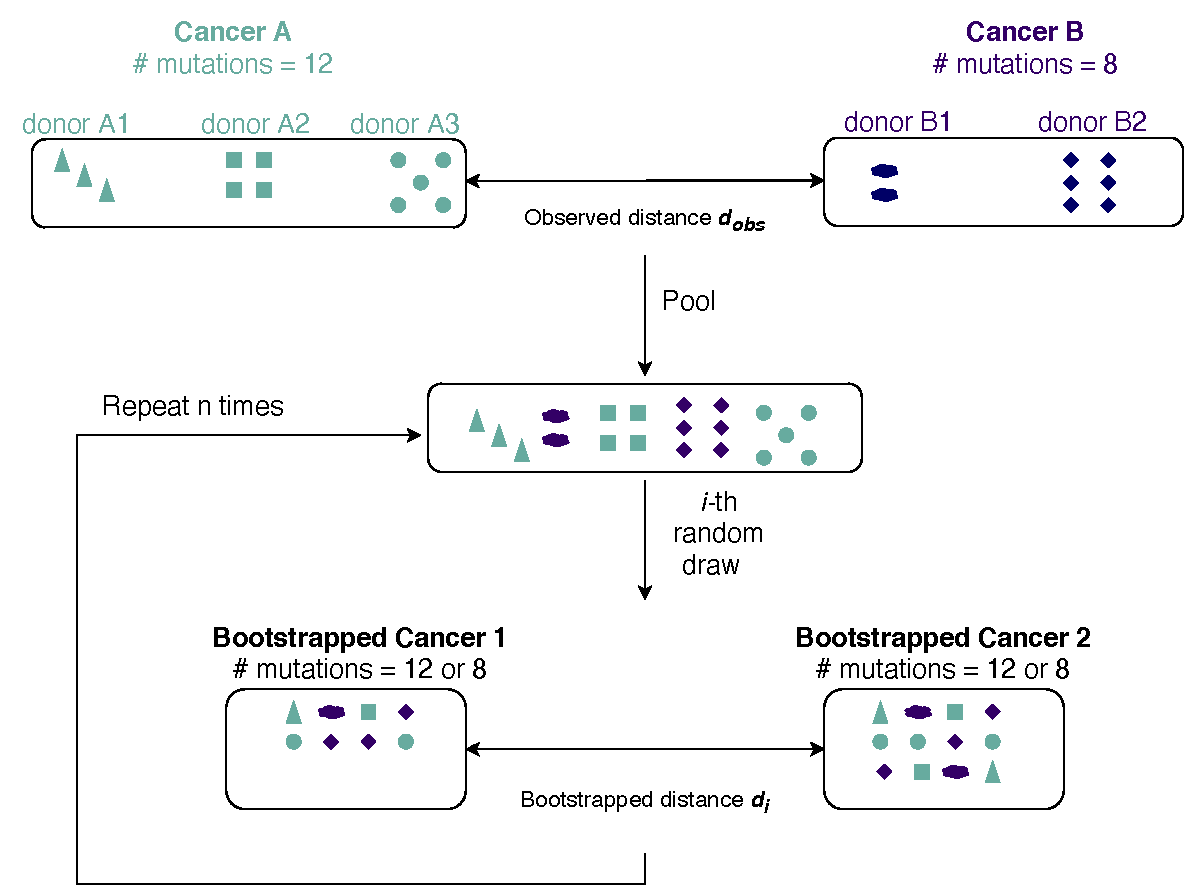
\includegraphics[scale=0.6]{graphics/bootstrap_demo.pdf}
    \caption{\textbf{Testing the hypothesis that two cancers share the same genomic distribution of mutations using bootstrap.} Mutations are pooled from 2 original cancers A and B, the distance between A and B is $d_{obs}$. 2 bootstrapped cancers 1 and 2 are then simulated by randomly drawing mutations from the pool, the number of mutations in 1 and 2 must be the same as either A or B. The distance $d_i$ between cancers 1 and 2 is then measured. This process is repeated 1000 times for each of the representations introduced. The estimated p-value is the number of times $d_i > d_{obs}$ divided by $n$.}
    \label{fig:bootstrap_demo}
\end{figure}


\section{Whole disease analysis of SCE}\label{methods:sce}
Cancers are known to have distinctive compositions of mutations, which themselves consist of two components: the base substitution and the flanking bases. Together, the two components are called sequence context effect (SCE). This section describes the statistical techniques  to measure the information content available in both components.

\subsection{Overview of the techniques to measure information}
The nature of SCE for both the base substitutions and the flanking bases is simply count data determined by categorical variables, which can be displayed on a contingency table. It is straightforward to assign this type of data to have a multinomial distribution. To establish whether or not one categorical variable (\textit{e.g.} the cancers) is deterministic of another (\textit{e.g.} the types of mutations), we can assume product multinomial sampling. Due to the mathematical connection between the product multinomial and Poisson distributions, one could execute this  via a generalised linear model (GLM) under the Poisson distribution \citep{Nelder1974LOGSQUARES.}. This project used the MutationMotif package previously developed in the Huttley lab, whose key function is \texttt{glm} from R \citep{Zhu2017}.

\subsubsection{Generalised linear model}
Table \ref{tab:glm_demo} illustrates how GLM can be used to evaluate whether one categorical variable is predictive of another. Specifically, the example tests whether the composition of base substitutions from the wildtype \textbf{T} differs for cancer A and B. Answering this question requires a null model ($H_o$) that assumes no relationship and a saturated model ($H_a$) that assumes an association between cancer types ($\lambda_{cancer}$) and the substitution types ($\lambda_{sub}$). This association manifests through the $\lambda_{cancer:sub}$ that is present in $H_a$ but absent in $H_o$. By measuring the deviance statistic $D$ (equation \ref{eq:deviance}), \textit{i.e.} how much information the null is missing from the saturated model, and contrasting $D$ against the $\chi^2$ distribution, a p-value can be obtained. A small enough p-value (usually $<0.05$) is taken to imply that $\lambda_{cancer}$ is predictive of $\lambda_{sub}$.

\begin{equation}
D = -2 \ln \frac{\hat{L}(saturated)}{\hat{L}(null)}
\label{eq:deviance}
\end{equation}
where $D$ is the deviance statistic; $\hat{L}$ is the estimated maximum likelihood for the parameters in the corresponding models.

\begin{figure}[h!]
  \begin{minipage}[c]{0.5\textwidth}
    \captionof{table}{\textbf{Example of how GLM and RE can be used for categorical data in a contingency table}. In this example, the categorical variable for cancer type $\lambda_{cancer}$ takes values cancer A or cancer B; the variable for the composition of base substitution $\lambda_{sub}$ takes values T$\rightarrow$A, T$\rightarrow$C and T$\rightarrow$G. To establish whether $\lambda_{cancer}$ is explanatory of $\lambda_{sub}$, one can perform a hypothesis test based on a null and a saturated model (formulae \ref{eq:spectra_demo}; the $counts$ corresponds to the $count$ term in equation \ref{eq:spectra_demo}). The hypothesis test outputs a p-value; if p-value is small enough, it can the explanatory relationship. The test also allows estimating $RE$, which measures how much information is contributed by each entry in the table.} 
    \label{tab:glm_demo}
  \end{minipage}\hfill
  \begin{minipage}[c]{0.48\textwidth}
    \begin{tabulary}{\columnwidth}{rRRR}
    \toprule
        & \textbf{T$\rightarrow$A} & \textbf{T$\rightarrow$C} & \textbf{T$\rightarrow$G}  \\
    \hline
        \textbf{Cancer A} & $count_{T>A}$ & $count_{T>C}$ & $count_{T>G}$  \\
        \textbf{Cancer B} & $count_{T>A}$ & $count_{T>C}$ & $count_{T>G}$  \\
    \bottomrule
    \end{tabulary}
    \vspace{1cm}
    \begin{equation}
        \begin{aligned}
            H_o: \ln{count} =& \lambda_{cancer} + \lambda_{sub}  & \\
            H_a: \ln{count} =& \lambda_{cancer} + \lambda_{sub} + \lambda_{cancer:sub}
        \end{aligned}
        \label{eq:spectra_demo}
    \end{equation}
  \end{minipage}
\end{figure}


\subsubsection{Relative entropy}\label{methods:re}
To measure the amount of information contributed by each entry in the contingency table ($count$ in Table \ref{tab:glm_demo}), I used relative entropy ($RE$). $RE_i$ for the entry $i$ can be calculated via the deviance residual $r_i$ of the entry \citep[$r_i$ obtained using appendix equation \ref{eq:dev_res};][]{Zhu2017}, as follows

\begin{equation}
    RE_i = \frac{r_i}{2n} 
    \label{eq:re}
\end{equation}
where $RE_i$ is the relative entropy for entry $i$ of the contingency table; $r_i$ is its deviance residual and $n$ is the total counts. 

Note that while the deviance $D$ measures the departure of the null from the saturated, $r_i$ is the contribution from entry $i$ to this departure, and the sum of all $r_i^2$ is equal to $D$. I chose $RE$ to be the measure of information because it scales the deviance residuals by its sample size, thereby making comparison across hypothesis tests with different amount of data valid. It is calculated as follows

\subsection{Base substitutions}\label{methods:spectra}
\subsubsection{Composition of base substitutions for individual cancers}
To examine the patterns of base substitution in a cancer, I calculated the $RE$'s when comparing that cancer to a ``null cancer'', where all mutation counts are the same (Table \ref{tab:glm_spectra}). Due to the difference in the abundance of nucleotides (\textit{e.g.} only about 41\% of the human genome is C+G, the rest is A+T), I separately calculated four $RE$ sets for substitutions that involved different wildtype bases. Table \ref{tab:glm_spectra} illustrates the set whose wildtype base is T. The results for this are available in Subsection \ref{sce:spectra}.

\vspace{0.2cm}
\begin{figure}[h!]
  \begin{minipage}[c]{0.4\textwidth}
    \captionof{table}{\textbf{Contingency table to examine the composition of base substitutions in Cancer A}. Cancer A is compared to a null cancer where all counts are the same. The resulting $RE$'s represent the excess/deficit of certain substitutions. This particular table computes the $RE$ set for substitutions whose wildtype is T. $\lambda_{cancer}$ is a categorical variable taking values \textbf{Cancer A} or \textbf{Null}. $\lambda_{sub}$ indicates whether the counted substitution is \textbf{T$\rightarrow$A}, \textbf{T$\rightarrow$C} or \textbf{T$\rightarrow$G}. For each cancer, three similar tables are required for substitutions of A, C and G.} 
    \label{tab:glm_spectra}
  \end{minipage}\hfill
  \begin{minipage}[c]{0.59\textwidth}
    \begin{tabulary}{\columnwidth}{lCCCR}
    \toprule
        & \textbf{T$\rightarrow$A} & \textbf{T$\rightarrow$C} & \textbf{T$\rightarrow$G}  & \textbf{total} \\
    \hline
        \textbf{Cancer A} & $count_{T>A}$ & $count_{T>C}$ & $count_{T>G}$ & $count_{tot}$ \\
        \textbf{Null} & $count_{tot}/3$ & $count_{tot}/3$ & $count_{tot}/3$ & $count_{tot}$ \\
    \bottomrule
    \end{tabulary}
    \vspace{0.9cm}
    \begin{equation}
        \begin{aligned}
            H_o: \ln{count} =& \lambda_{cancer} + \lambda_{sub}  & \\
            H_a: \ln{count} =& \lambda_{cancer} + \lambda_{sub} + \lambda_{cancer:sub}
        \end{aligned}
        \label{eq:spectra}
    \end{equation}
  \end{minipage}
\end{figure}


\subsubsection{Base substitutions across cancers}
Having looked at the base substitutions for individual cancers, I examined how well base substitutions can be used to discriminate cancers. To compare two cancers, the contingency table for this analysis is similar to the example in Table \ref{tab:glm_demo}. Similar to the case of individual cancers, I analysed mutations from different wildtype bases separately using the so-called mutation spectrum test of \citet{Zhu2017}. In addition to the $RE$'s, also looked at the p-values from the hypothesis tests. Since there are four hypothesis tests, there are four p-values, which I combined these p-values into one p-value using the Fisher's method \citep[details in \ref{apdx:fisher};][]{Fisher1992StatisticalWorkers}. Briefly, Fisher's method adds up all the logs of the member p-values, this value is doubled and contrasted against the $\chi^2$ distribution to obtain the final joint p-value. 66 joint p-values were obtained and adjusted using Bonferroni multiple test correction \citep[equation \ref{eq:bonferroni};][]{Armstrong2014WhenCorrection}.

\subsection{Flanking bases}\label{methods:nbr}
In this subsection, we are interested in the information content available in the flank base component of SCE, including positions -1, +1, -2 and +2 with respect to the mutation. This is the neighbour analysis from \citet{Zhu2017}. As for the base substitution analyses, I separated the analysis for different mutations due to their different frequencies of occurrence. Figure \ref{fig:nbr_demo} illustrates how information can be measured for position +1 of the C$\rightarrow$T mutation in some cancer A. Specifically, the analysis measures the extent to which bases found next to the C$\rightarrow$T mutation tend to differ from bases next to a randomly selected C in the genome. To do this, for each C$\rightarrow$T substitution, a random C within the neighbourhood of 500 bases to each side of the substitution was selected and its flanking base at position +1 was recorded. I then received a contingency table. Using the models in formulae \ref{eq:nbr_demo}, I obtained the $RE$'s, as described in subsection \ref{methods:re}, whose total is the desired measure of information. I measured the total $RE$ for all other flank positions of the 5-mer context and all other mutations.

\begin{figure}[h!]
  \begin{minipage}[c]{0.48\textwidth}
    \caption{
      \textbf{The smoothing approach is expected to be more robust than the bin approach.} Both panels depict the same mutation location data for a hypothetical chromosome, with the black dots below the x-axis representing the true location of mutations. By binning the genome by convention, one counts the number of mutations in each green bin. The obtained GLE data is then the green dots on top of each bin. This binned GLE data changes when shifting the bin boundaries from panel (a) to panel (b). On the contrary, the smooth representation of GLE, which adopts \gls{density} estimation, is depicted by the purple dots on the purple line. By smoothing the genome, GLE data is the same for both panels. 
    } \label{fig:mutdistribution_demo}
  \end{minipage}\hfill
  \begin{minipage}[c]{0.55\textwidth}
    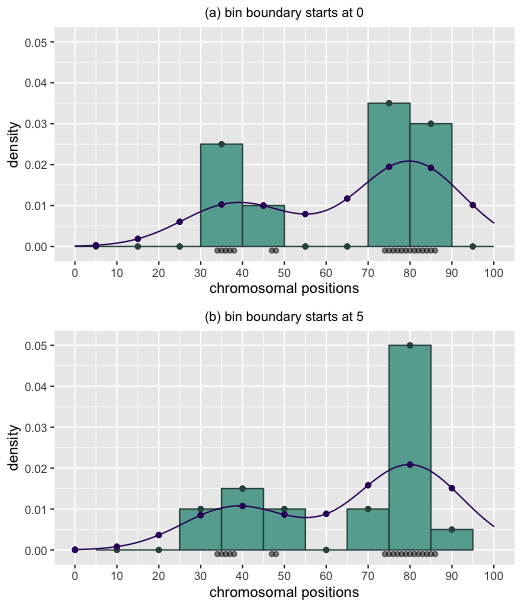
\includegraphics[width=\textwidth]{graphics/mutdistribution_demo.png}
  \end{minipage}
\end{figure}


\section{Mutation-based classifier for cancers}\label{methods:ml}
Based on the premise that GLE and SCE are important aspects of a cancer mutation profile, this section explores how we could exploit the information from GLE and SCE for cancer classification. Because I trialled different approaches to represent data, I expect the known properties of the best performing approach should reveal important characteristics of the data. More critically, it should validate the findings from whole disease analyses, thereby consolidating our understanding of cancer mutagenesis.

\subsection{Machine learning workflow}\label{methods:ml_workflow}
For all classifiers trained in the subsequent subsections, I followed the same training procedures \citep{Zengyou2015DataApplications}. 

\subsubsection{$K$-nearest neighbours}
One algorithm that uses pairwise distances between observations to describe both GLE and SCE is the $K$-nearest neighbours \citep[KNN;][]{Neath2010DiscriminationClassification}. There are two reasons there was a preference for distances over raw feature vectors (\textit{i.e.} the bin/smooth vector of density for GLE or the mutation count vector for SCE). First, as in the case for most biological data, our data suffered from the curse of dimensionality \citep{Banks2003DataStatistics}, meaning there were more parameters than there were observations, making inference less robust. For example, the bin representation for GLE alone has about 3000 parameters corresponding to $\approx$3000 bins, while there are only about hundreds of donors available. Describing data in terms of distances is therefore a way to escape the curse of dimensionality (training $\approx$3000 parameters on a few hundred observations). Second, I was interested in experimenting with different types of metrics that might better describe the data than the typically default Euclidean distance, such as the Wasserstein and Jensen-Shannon distance. The principle of the KNN algorithm is straightforward (Figure \ref{fig:knn_demo}). The input into the classifier is a pairwise distance matrix between all donors. When prediction on an unknown donor needs to be made, KNN calculates the distances from the unknown to all known donors in the training set and identifies the nearest training points (known neighbours) to the unseen donor. The predicted cancer will be the predominant cancer within these neighbours. This was done using \texttt{sklearn.neighbors.KNeighborsClassifier} \citep{scikit-learn}.

\begin{figure}[ht!]
    \centering
    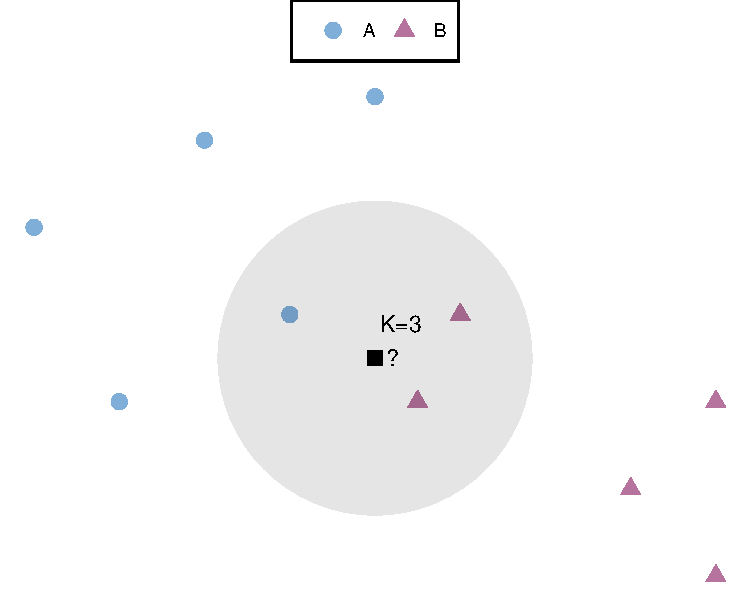
\includegraphics[scale=0.8]{graphics/knn_demo.pdf}
    \caption{\textbf{Illustration of K-nearest neighbours (KNN) algorithm.} When K=3, 3 neighbours to the new donor are identified based on the pre-calculated distances. The 3 neighbours get to ``vote'' for the prediction made on the new donor. Because there are 2 B's and 1 A, the new donor has cancer B.}
    \label{fig:knn_demo}
\end{figure}


\newpage
\subsubsection{F1-score}
I used F1-score to measure the accuracy of the models in the validation step \citep{Kulkarni2020FoundationsDemocracy}. $F1$ is a typically recommended measure of accuracy as it is the combination of sensitivity and specificity of the predictions (equation \ref{eq:f1}). Taking Cancer A as an example, sensitivity refers to how well a model can recognise Cancer A (equation \ref{eq:sensitivity}), and specificity refers to how likely a sample is Cancer A if it is predicted to be Cancer A (equation \ref{eq:specificity}). To get the overall $F1$ for the model, I calculated $F1$ for each cancer and averaged them, weighing by the true instances in each cancer.

\begin{equation}
    F1 = 2\frac{sensitivity \times specificity}{sensitivity + specificity}    
    \label{eq:f1}
\end{equation}

\subsubsection{Cross validation}
Training a KNN classifier where inputs are distances, as in our case, simply means choosing the number of neighbours $K$ used for prediction. This process is also called hyper-parameter tuning, illustrated in Figure \ref{fig:cv_demo}. Specifically, I saved 1/10 of the data to be the test set. I then split the remaining training set (9/10 of the data) into five folds (or sections). Note that the proportions of different cancers were the same for all splits. The first four folds were visible to the model and are called the training set; meanwhile, the 5$^{th}$ fold was not seen by the model and is called the validation set. The ``$K$'' in KNN represents the number of neighbouring observations used for prediction. I trialled $K$ from 1 to $n$, where $n$ was the number of donors available in the cancers with fewest donors in the validation set. By contrasting the prediction made by the test set against the validation set, each trial outputs an $F1$. I then repeated the 5-fold cross validation procedure by sequentially replacing the 5$^{th}$ fold with the other folds. Eventually, I was able to pick the $K$ with the highest average $F1$. I then applied this $K$ to the test set to obtain the final $F1$. The whole process was repeated 10 times to establish a sense of variation in the final accuracy evaluation.

\begin{figure}[h!]
    \centering
    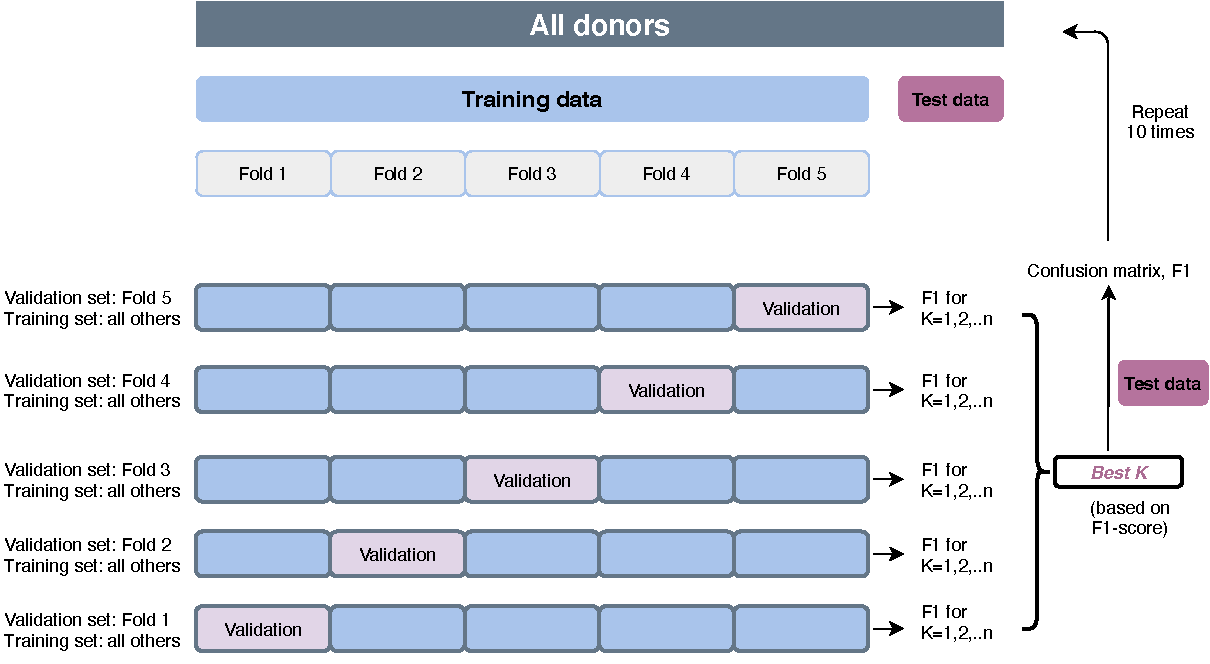
\includegraphics[scale=0.78]{graphics/ML_demo.pdf}
    \caption{\textbf{Illustration of machine learning cross validation workflow.} Data was split into a test set (1/10) and a training set (9/10). The training set was divided into 5 folds, each fold was sequentially used as a validation set to select the parameter $K$ of the model. From the set of $F1$'s for each $K$, I selected the best $K$. This $K$ was then applied to the test set for final evaluation (1/10 of the data). The whole process was repeated 10 times to evaluate the possible range of the accuracy, reported in the form of confusion matrices or $F1$.}
    \label{fig:cv_demo}
\end{figure}


\subsection{Classifier by GLE}
To classify cancers based on GLE, I experimented with two representations: bin \& smoothing and two distance measures: Euclidean \& Wasserstein distance. Details about the techniques of these representations and measures have been described in subsection \ref{methods:bootstrap}. The difference is that this section is on the individual donor scale. Briefly, for each donor, GLE was represented in the form of either the bin or the smoothing approach. For each representation, Euclidean or Wasserstein distances were then calculated for each pair of donors. The classifier was then trained as per the procedure outlined above. The results for this are available in Section \ref{ml:gle} of Chapter \ref{ml}.

\subsection{Classifier by SCE}\label{methods:ml_sce}
In this subsection, I trialled different representations of SCE, all representations used the Jensen-Shannon distance. 

\subsubsection{Jensen-Shannon distance}
I used Jensen-Shannon distance \citep[JSD;][]{Osterreicher2003} as the measure of distance to classify cancers based on SCE. JSD is an appropriate measure for composition data like SCE because it gives weights to the more dominant elements. For example, the contribution of C$\rightarrow$T mutations to the JSD between two donors depends on both the difference in  C$\rightarrow$T and the abundance of C$\rightarrow$T in the two donors. Additionally, JSD is the symmetric version of the Kullback-Leibler divergence \citep{Kullback1951}. It is calculated as follows:

\begin{equation}
    d_{JS}(P,Q) = \sqrt{\frac{1}{2} (d_{KL}(P|M) + d_{KL}(Q|M))}
\end{equation}
where $d_{JS}(P,Q)$ is the JSD between the SCE of donors P and Q; M is the average between P and Q: $M = \frac{P+Q}{2}$; $d_{KL}(P|M)$ is the Kullback-Leibler divergence of M from P, likewise for Q. $d_{KL}$ can be calculated as per equation \ref{eq:kl} in the appendix.

The representations of the vectors to train the KNN classifier based on JSD are described below.

\subsubsection{Comparing 1-mer, 3-mer and 5-mer}
Due to SCE's nature as composition data, one obvious way to represent SCE is the proportion of mutations. To be precise, the vector that represents SCE for a donor is the count of different mutation types, divided by the total number of mutations. The generation of the count vector is illustrated in Figure \ref{fig:get_sce}. However, it is worth noting that as the k-mer size increases, the number of elements in the SCE vector increases very rapidly, according to equation \ref{eq:sce_counts} (Figure \ref{fig:sce_size}).

\begin{figure}[ht!]
    \begin{subfigure}{\textwidth}
    \centering
    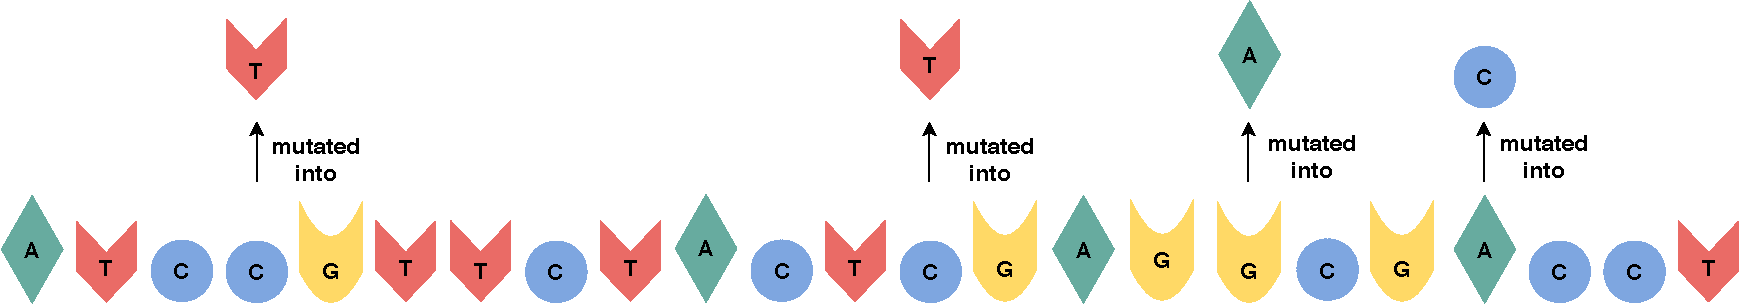
\includegraphics[scale=0.5]{graphics/sce_counts.pdf} \\
    \vspace{0.9cm}
    \begin{tabulary}{\columnwidth}{cc|cc|cc}
    \toprule
        \multicolumn{2}{c}{\textbf{1-mer}}  & \multicolumn{2}{c}{\textbf{3-mer}} & \multicolumn{2}{c}{\textbf{5-mer}} \\
        \hline
        mutation & count vector & mutation & count vector & mutation & count vector \\
    \hline
        [A$\rightarrow$C] & 1 & G[A$\rightarrow$C]C & 1 & CG[A$\rightarrow$C]CC & 1 \\
        
        [C$\rightarrow$T] & 2 & C[C$\rightarrow$T]G & 1 & TC[C$\rightarrow$T]GT & 1 \\
        
         &  & T[C$\rightarrow$T]G & 1 & CT[C$\rightarrow$T]GA & 1 \\
         
        [G$\rightarrow$A] & 1 & G[G$\rightarrow$A]C & 1 & AT[G$\rightarrow$A]CG & 1 \\
        
        ... & 0 & ... & 0 & ... & 0 \\
    \bottomrule
    \end{tabulary}
    \caption{Generating the count vector for 1-mer, 3-mer and 5-mer}\label{fig:get_sce}
    \end{subfigure} \\

  \vspace{1cm}
  \begin{subfigure}{\textwidth}
  \begin{minipage}{0.65\textwidth}
    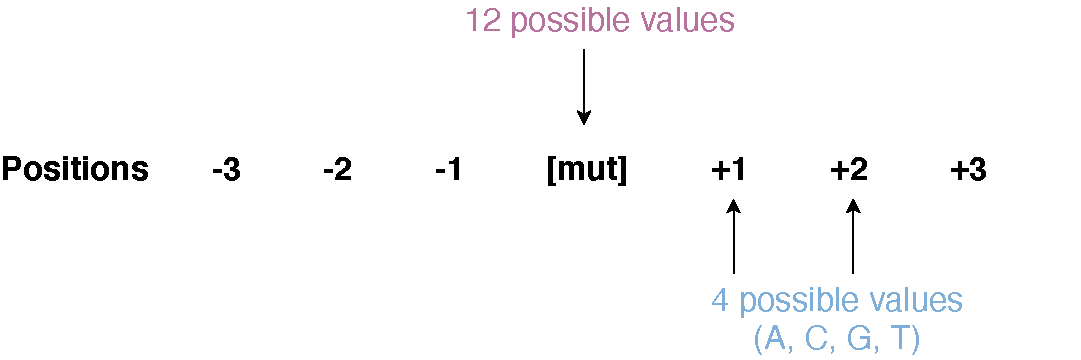
\includegraphics[width=\textwidth]{graphics/sce_counts_demo.pdf}
  \end{minipage}
  \begin{minipage}{0.3\textwidth}
    \begin{equation}
    l = 12 \times 4^{k-1}
    \label{eq:sce_counts}
    \end{equation}
    where $l$ is the number of elements and $k$ is the k-mer size, so $k-1$ is the number of flanking bases involved
  \end{minipage}
    \caption{Total number of elements for SCE incorporating flanking positions}\label{fig:sce_size}
  \end{subfigure} \\
  \vspace{0.2cm}
  \caption{
%   \textbf{The number of elements increases extremely rapidly with increasing k-mer size.} This is because there are 12 possible mutations, and for each flanking position, there are 4 possible bases. Panel (a) gives an example of how the count vector for SCE is generated for 1-mer, 3-mer and 5-mer for a DNA sequence with 4 mutations. The elements in the count vector were then divided by the total number of mutations to obtain the SCE vector. Panel (b) illustrates how to calculate the number of elements given the $k$-mer size. 
} \label{fig:sce_counts}
\end{figure}


\subsubsection{Strand asymmetric, semi-symmetric and fully-symmetric representations}
The rapid growth in the number of mutations when incorporating more flanking positions inevitably results in sparse vectors with many 0 values, as some donors only have hundreds of mutations. Accordingly, I investigated whether introducing strand symmetry, at the expense of some information loss, could address this issue. Therefore, this analysis could also reveal a mechanism of mutagenesis in cancer, which is whether mutation strand symmetry exists or not. There are three levels of strand symmetry involved, asymmetry, semi-symmetry and full-symmetry. Specifically, asymmetry is the normal mutation counts described above. For semi-symmetry, as described in Figure \ref{fig:motif_symmetric_demo}, whatever mutations that start with G or T were counted as part of the mutations on their reverse complementary strand. This is the representation adopted by the common literature such as \citet{Jiao2020}. The fully symmetric representation is even more stringent, it restricts the alphabet of the flanking bases to be A and C rather than A, C, T and G. This means that on the flanking base components, T was counted as A and G was counted as C. Table \ref{tab:sce_symmetric} summarises the properties of the three representations.

\begin{table}[ht!]
\centering
\caption{}
% \caption{\textbf{Summary of the number of elements available in the vectors for three levels of strand symmetry imposed on SCE.} Similarly to equation \ref{eq:sce_counts}, $l$ is the number of elements in the SCE vector, $k$ is the k-mer size}
\label{tab:sce_symmetric}
\begin{tabulary}{\textwidth}{ lrrr }
\toprule
 & \textbf{asymmetry} & \textbf{semi-symmetry} & \textbf{full-symmetry} \\
 $k$(-mer) & $l = 12 \times 4^{k-1}$ & $l = 6 \times 4^{k-1}$ & $l = 6 \times 2^{k-1}$ \\
\hline

1 & 12 & 6 & 6 \\
3 & 192 & 96 & 24 \\
5 & 3072 & 1536 & 96 \\

\bottomrule

\end{tabulary}
\end{table}


\subsubsection{Dissecting the 5-mer sequence context}
A second approach to reduce the sparsity of large sequence contexts (in this case 5-mer), without loss of information, is to dissect them into smaller submotifs. Specifically, instead of one count vector that incorporates all substitutions flanking positions of 5-mer, I computed multiple submotif vectors that incorporate 1 (2-submotif) or 2 (3-submotif) flanking positions with the mutations. A summary of these representations is presented in table \ref{tab:submotif}. While my previous approaches approaches used one single type of vector to generate a single pairwise distance matrix. The approach in this subsection computed pairwise distance matrices for all submotif vectors, and amalgamated these matrices by averaging all their elements. The resulting pairwise distance matrix was used to train the classifier for submotifs. 

\begin{table}[hp!]
\centering
\caption{\textbf{Summary of the properties of the representations that dissect 5-mer into smaller submotifs.} 2-submotif has 4 component vectors; 3-motif has 3 component vectors. \textbf{\#elements} are the number of elements available in each component vector.}
\label{tab:submotif}
\begin{tabulary}{\textwidth}{ lllllL }
\toprule
 & \textbf{vector 1} & \textbf{vector 2} & \textbf{vector 3} & \textbf{vector 4} & \textbf{\#elements} \\
\hline
2-submotif & (mut, pos-2) & (mut, pos-1) & (mut, pos+1) & (mut, pos+2) & 48 \\
3-submotif & (mut, pos-2,-1) & (mut, pos-1,+1) & (mut, pos+1,+2) & & 192 \\
whole-5mer & (mut, all 4 pos) & & & & 3072 \\
\bottomrule
\end{tabulary}
\end{table}


\subsection{Combining GLE with SCE in a joint classifier}\label{methods:ml_both}
Because GLE and SCE are distinct types of information, in this section, I attempted to combine the two factors to see if it could further improve the predictive power compared to each factor by itself.

\subsubsection{Kernel normalisation}
GLE and SCE have different units, leading to the need to normalise them. By normalising the data, the joint classifier can simultaneously avoid one factor being dominated by the other purely due to their mismatched numerical scales and assess which factor was the stronger predictor of cancer type. For each factor, the normalisation step was done while converting its pairwise distance matrix into a pairwise kernel matrix. It is worth noting that intuitively, the distance matrix measures the difference between data points and kernel matrix measures the similarity between them. I used the Laplacian kernel function for each element of the distance matrix \citep{Wang2016ApplicationFunction}, as follows:

\begin{equation}
    k(x,y) = \exp\bigg( - \frac{d(x,y)}{\sigma}\bigg)
    \label{eq:laplacian}
\end{equation}
where $k$ is an entry of the resulting kernel matrix corresponding to the pair of data points (\textit{i.e.} donors) $x$ and $y$; $d(x,y)$ is the distance between $x$ and $y$ in the distance matrix; $\sigma$ is intuitively the scale parameter. I set $\sigma$ as the median of the distance matrix, excluding the case where $x$ and $y$ were the same. The division by $\sigma$ ensured that the distances in the normalised matrices were numerically on the same scale.

After the normalisation step, I obtained a normalised pairwise kernel matrix $G$ for GLE and $S$ for SCE.

\subsubsection{Weighted combination of GLE and SCE}
I trialled different weights on the linear combination of the kernel matrices $G$ and $S$ according to equation \ref{eq:joint}

\begin{equation}
    J = gG + (1-g)S
    \label{eq:joint}
\end{equation}
where $J$ is the joint kernel matrix; $G$ and $S$ are the kernel matrices for GLE and SCE; $g$ is the weight given to $G$, $1-g$ is the weight given to $S$, $g$ and $1-g$ take values 0, 0.1, 0.2,..., 1. I then converted the joint kernel matrix $J$ into a joint distance matrix $D_J$ using the standard generic approach \citep[more in the appendix equation \ref{eq:k2d_ori};][]{Phillips20112Distance}

\begin{equation}
    d_J(x,y) = \sqrt{2 - 2k(x,y)}
    \label{eq:k2d}
\end{equation}
where $d_J(x,y)$ is the entry for $x$ and $y$ to the joint distance matrix $D_J$; $k(x,y)$ is the entry to the joint kernel matrix $J$.

The subsequent training step proceeded as described in subsection \ref{methods:ml_workflow}. Figure \ref{fig:joint} summarises the procedure for training the joint classifier.

\begin{figure}[ht!]
    \centering
    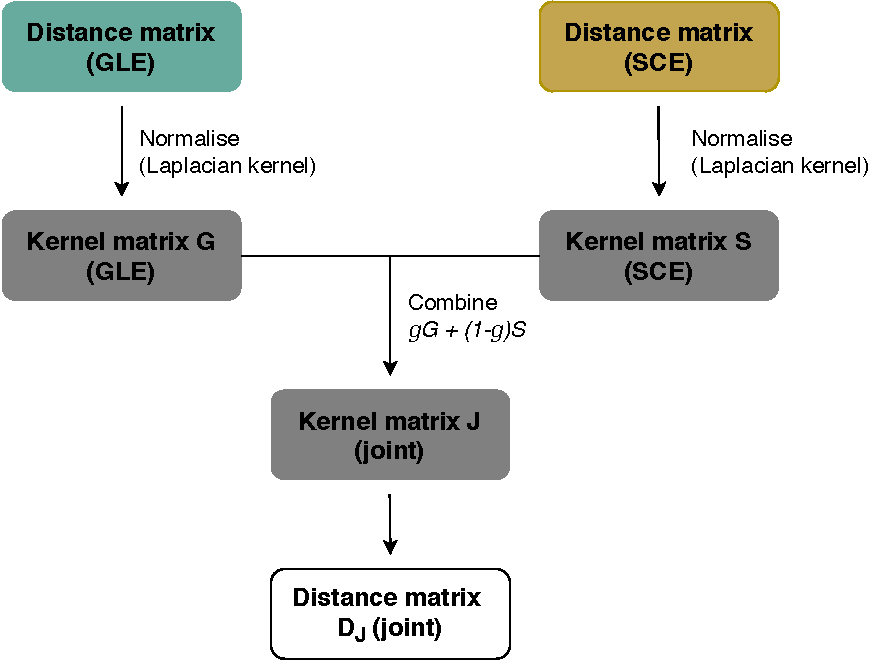
\includegraphics[scale=0.8]{graphics/joint_classifier.pdf}
    \caption{\textbf{Summary of the methods to train the joint classifier for GLE and SCE}. The pairwise distance matrix for each factor was converted to a kernel matrix, normalised and linearly combined with weights $g$ and $1-g$ to get the joint kernel matrix $J$ (equation \ref{eq:joint}). $J$ was then converted back to a distance matrix $D_J$ using equation \ref{eq:k2d}. $D_J$ was subsequently used for model training.}
    \label{fig:joint}
\end{figure}


